\begin{center}
\captionsetup{type=figure}
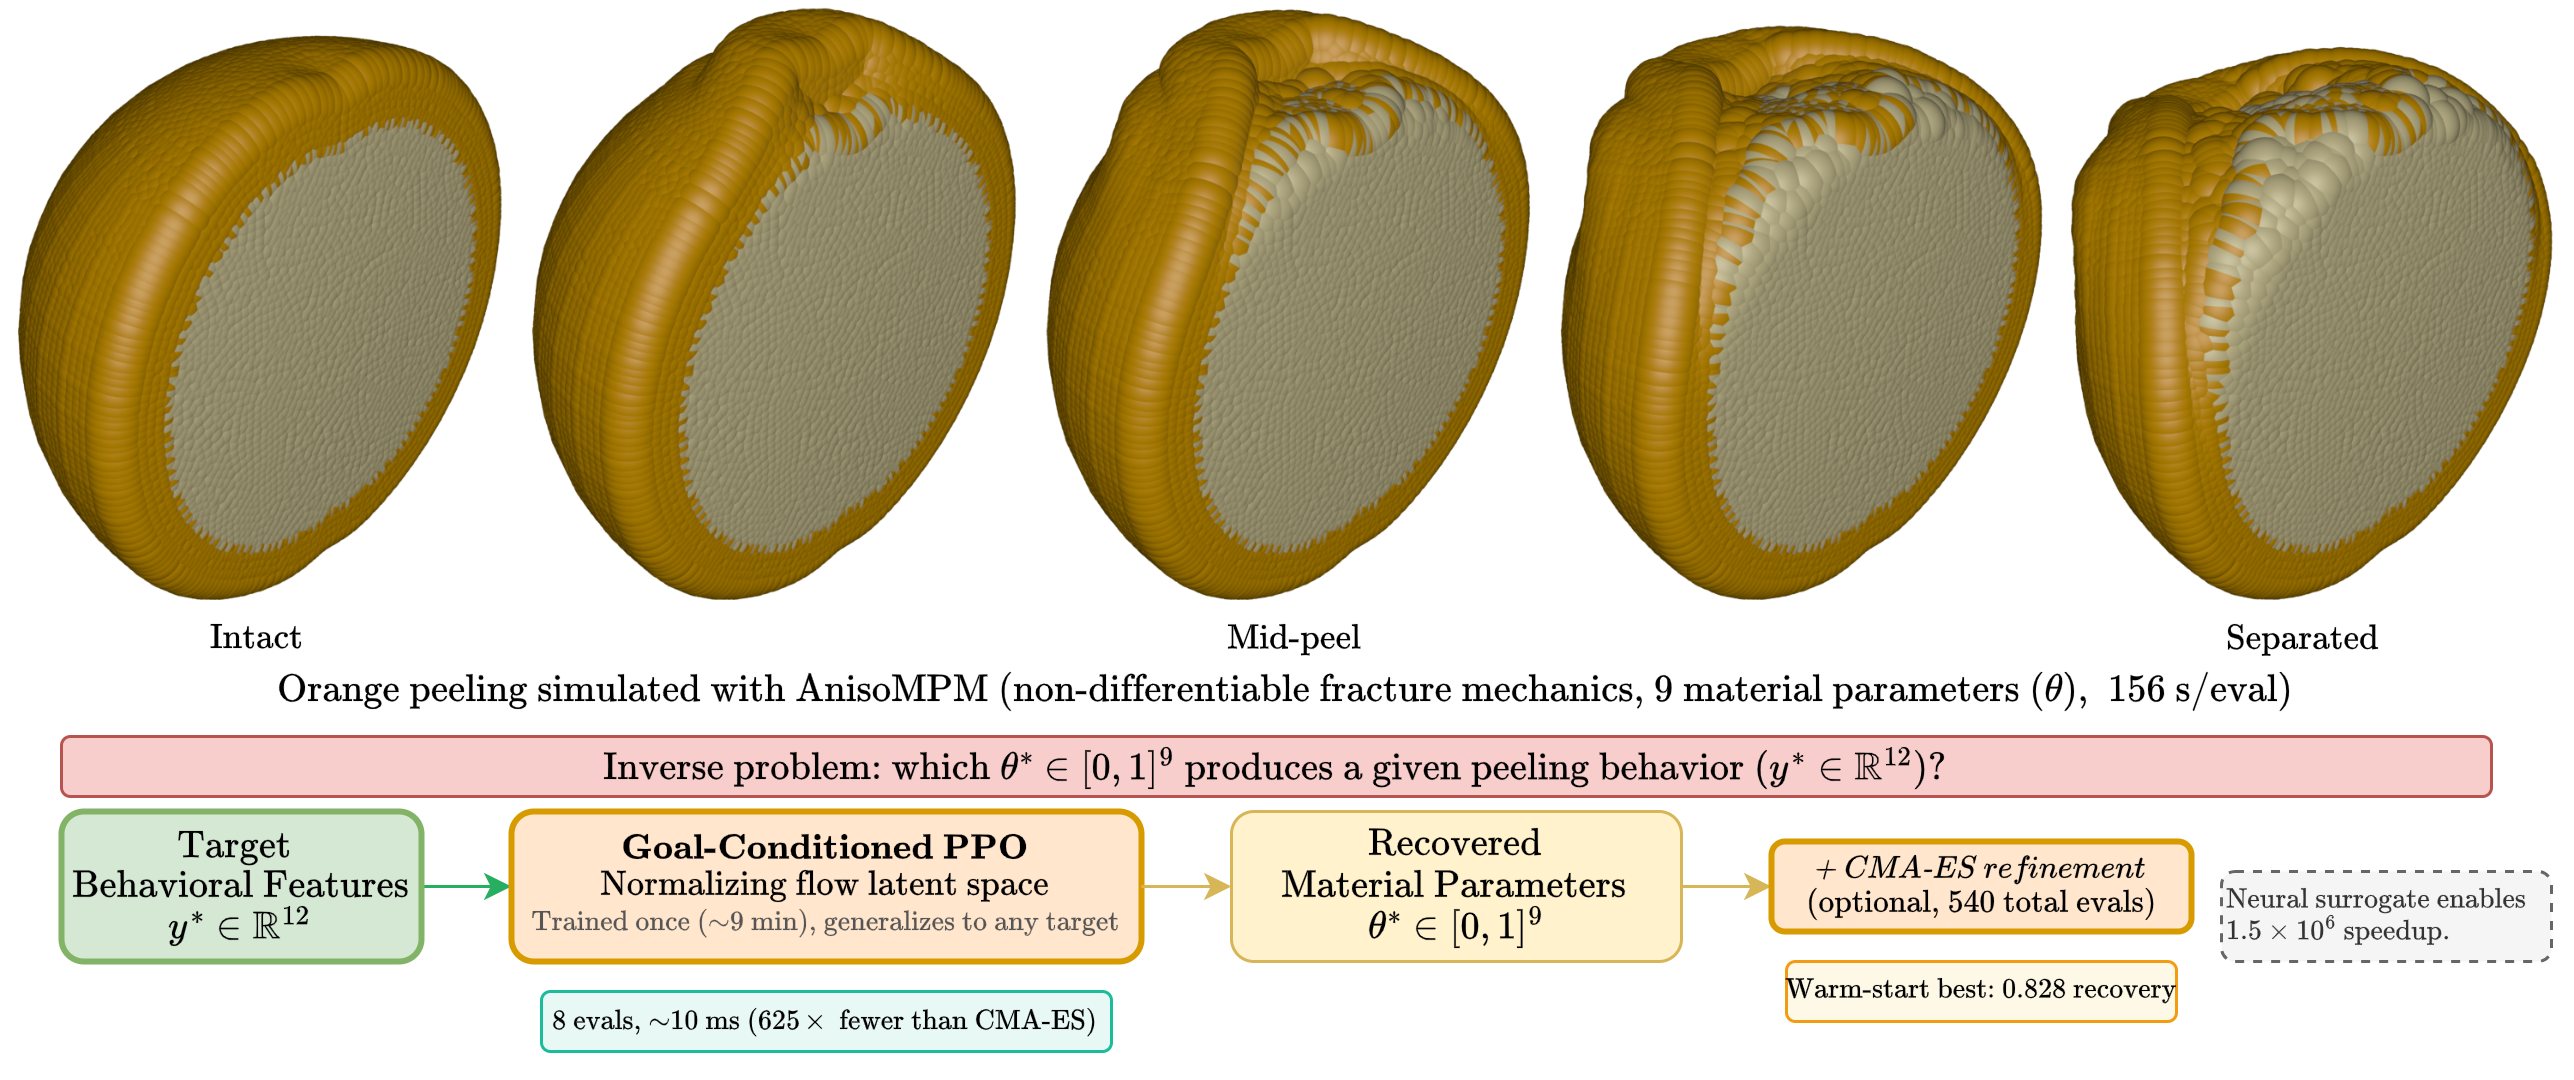
\includegraphics[width=1.0\textwidth]{media/teaser.png}
% \fbox{\parbox{0.95\textwidth}{\centering\vspace{2em}
% \vspace{2em}}}
\captionof{figure}{Orange peeling simulated with AnisoMPM~\cite{wolper2020anisompm}, a non-differentiable fracture mechanics simulator with $9$ material parameters and ${\sim}156$\,s per evaluation. Different parameter settings produce qualitatively different peeling behaviors. Our inverse estimation pipeline. Given target behavioral features $\mathbf{y}^*$ describing a desired peeling outcome, a goal-conditioned PPO policy operating in a normalizing flow latent space recovers the material parameters $\boldsymbol{\theta}^*$ in $8$ surrogate evaluations (${\sim}10$\,ms), $625\times$ fewer than CMA-ES. The policy is trained once (${\sim}9$\,min) and generalizes to arbitrary targets without retraining. A neural surrogate provides a $1.5{\times}10^6$ speedup over the simulator, and optional CMA-ES warm-start refinement ($540$ total evaluations) pushes recovery to $0.828$.}
\label{fig:teaser}
\end{center}